\documentclass[
    12pt, % Schriftgröße
    DIV10,
    ngerman, % für Umlaute, Silbentrennung etc.
    a4paper, % Papierformat
    oneside, % einseitiges Dokument
    titlepage, % es wird eine Titelseite verwendet
    parskip=half, % Abstand zwischen Absätzen (halbe Zeile)
    headings=normal, % Größe der Überschriften verkleinern
    listof=totoc, % Verzeichnisse im Inhaltsverzeichnis aufführen
    bibliography=totoc, % Literaturverzeichnis im Inhaltsverzeichnis aufführen
    index=totoc, % Index im Inhaltsverzeichnis aufführen
    captions=tableheading, % Beschriftung von Tabellen unterhalb ausgeben
    final % Status des Dokuments (final/draft)
]{scrartcl}

% Pakete

% Schrift ----------------------------------------------------------------------
\usepackage{lmodern} % bessere Fonts

% Paket für Kopfzeilen und Fußzeilen
\usepackage[
    automark, % Kapitelangaben in Kopfzeile automatisch erstellen
    headsepline, % Trennlinie unter Kopfzeile
    ilines % Trennlinie linksbündig ausrichten
]{scrpage2}

% Anpassung an Landessprache
\usepackage[ngerman]{babel}

% Umlaute ----------------------------------------------------------------------
%   Umlaute/Sonderzeichen wie äöüß direkt im Quelltext verwenden (CodePage).
%   Erlaubt automatische Trennung von Worten mit Umlauten.
% ------------------------------------------------------------------------------
\usepackage[utf8]{inputenc}
\usepackage[T1]{fontenc}
\usepackage{textcomp} % Euro-Zeichen etc.

\usepackage[babel,german=quotes]{csquotes}

% Bei Änderungen müssen die *.aux und *.bbl Dateien manuell gelöscht werden
% Sonst kommt es zu einem Fehler bei der Erstellung
%\usepackage[round, sort, comma, numbers]{natbib}
%\usepackage[round, numbers]{natbib}
%\bibliographystyle{abbrvdin}
%

\usepackage{scrhack}

\usepackage[citestyle=alphabetic,bibstyle=alphabetic,backend=biber]{biblatex}
\bibliography{Bibliographie}
\DefineBibliographyStrings{german}{
  bibliography = {Literaturverzeichnis},
}
\setlength\bibitemsep{8pt}

\usepackage{xpatch}
\xpretobibmacro{author}{\mkbibbold\bgroup}{}{}
\xapptobibmacro{author}{\egroup}{}{}
\xpretobibmacro{editor}{\mkbibbold\bgroup}{}{}
\xapptobibmacro{editor}{\egroup}{}{}
\xpretobibmacro{editor+others}{\mkbibbold\bgroup}{}{}
\xapptobibmacro{editor+others}{\egroup}{}{}
\xpretobibmacro{bbx:editor}{\mkbibbold\bgroup}{}{}
\xapptobibmacro{bbx:editor}{\egroup}{}{}

% Grafiken ---------------------------------------------------------------------
% Einbinden von JPG-Grafiken ermöglichen
\usepackage[dvips,final]{graphicx}
\graphicspath{{Bilder/}}

% Paket zur Verwendung zusätzlicher Positionsbefehle
\usepackage{float}

% Befehle aus AMSTeX für mathematische Symbole z. B. \boldsymbol \mathbb --------
\usepackage{amsmath,amsfonts}

% Einfache Definition der Zeilenabstände und Seitenränder etc. -----------------
\usepackage{setspace}
\usepackage{geometry}

% zum Umfließen von Bildern ----------------------------------------------------
\usepackage{floatflt}

% Farbdefinitionen
\usepackage{xcolor} 
\definecolor{hellgelb}{rgb}{1,1,0.9}
\definecolor{colKeys}{rgb}{0,0,1}
\definecolor{colIdentifier}{rgb}{0,0,0}
\definecolor{colComments}{rgb}{1,0,0}
\definecolor{colString}{rgb}{0,0.5,0}
\definecolor{whgreen}{RGB}{113,177,41}
\definecolor{dvBlue}{RGB}{0,85,160}

% URL verlinken, lange URLs umbrechen etc. -------------------------------------
\usepackage{url}

% PDF-Optionen -----------------------------------------------------------------
\usepackage[
    bookmarks,
    bookmarksopen=true,
    colorlinks=true,
% diese Farbdefinitionen zeichnen Links im PDF farblich aus
    linkcolor=dvBlue, % einfache interne Verkn�pfungen
    anchorcolor=black,% Ankertext
    citecolor=dvBlue, % Verweise auf Literaturverzeichniseintr�ge im Text
    filecolor=magenta, % Verkn�pfungen, die lokale Dateien �ffnen
    menucolor=dvBlue, % Acrobat-Men�punkte
    urlcolor=dvBlue, 
% diese Farbdefinitionen sollten für den Druck verwendet werden (alles schwarz)
%    linkcolor=black, % einfache interne Verkn�pfungen
%    anchorcolor=black, % Ankertext
%    citecolor=black, % Verweise auf Literaturverzeichniseintr�ge im Text
%    filecolor=black, % Verkn�pfungen, die lokale Dateien �ffnen
%    menucolor=black, % Acrobat-Men�punkte
%    urlcolor=black, 
    %backref, % Inkompatibel mit BibLateX
    plainpages=false, % zur korrekten Erstellung der Bookmarks
    pdfpagelabels, % zur korrekten Erstellung der Bookmarks
    hypertexnames=false, % zur korrekten Erstellung der Bookmarks
    linktocpage % Seitenzahlen anstatt Text im Inhaltsverzeichnis verlinken
]{hyperref}

% fortlaufendes Durchnummerieren der Fußnoten ----------------------------------
\usepackage{chngcntr}
%\counterwithout{footnote}{chapter}

% Formatierung von Listen ändern -----------------------------------------------
\usepackage{paralist} % itemize, enumerate

% bei der Definition eigener Befehle benötigt
\usepackage{ifthen} % Vielleicht nicht nötig

% definiert u.a. die Befehle \ und \listoftodos
\usepackage{todonotes}
\reversemarginpar

% sorgt dafür, dass Leerzeichen hinter parameterlosen Makros nicht als Makroendezeichen interpretiert werden
\usepackage{xspace}

\usepackage{tabularx} % Tabellenspalten mit variabler Breite
\usepackage{wrapfig}  % Schriftumflossene Bilder


% Seitenstil

% Zeilenabstand 1,5 Zeilen
\onehalfspacing

% Seitenränder
% bottom is 20 + X, weil Footer nicht berücksichtigt wird
\geometry{paper=a4paper,left=30mm,right=20mm,top=20mm, bottom=38mm, footskip=8mm}

% Kopf- und Fußzeilen ----------------------------------------------------------
% Kopf- und Fußzeile auch auf Kapitelanfangsseiten
%\renewcommand*{\chapterpagestyle}{scrheadings} 
% Schriftform der Kopfzeile
%\renewcommand{\headfont}{\normalfont}

% Kopfzeile
\ihead{\headmark} % links
\chead{}
%\ohead{\includegraphics[scale=0.1]{Bilder/DJLogo.png}} % rechts
\setlength{\headheight}{20mm} % Höhe der Kopfzeile
% Kopfzeile über den Text hinaus verbreitern
%\setheadwidth[0pt]{textwithmarginpar} 
\setheadsepline[text]{0.4pt} % Trennlinie unter Kopfzeile

% Fußzeile
%\ifoot{} % links
\cfoot{} % mitte
\ofoot{\pagemark} % rechts
%\setfootsepline[text]{0.4pt} % Trennlinie unter Kopfzeile



% Schusterjungen und Hurenkinder vermeiden
%\clubpenalty = 10000
%\widowpenalty = 10000 
%\displaywidowpenalty = 10000

% Verringert den Abstand über den Überschriften
%\renewcommand*{\chapterheadstartvskip}{\vspace*{-\topskip}}

% Irgendwas mit Silbentrennung in MonoSpace (texttt)
\newcommand{\origttfamily}{}% sollte noch nicht definiert sein!
\let\origttfamily=\ttfamily % alte Definition von \ttfamily sichern
\renewcommand{\ttfamily}{\origttfamily \hyphenchar\font=`\-}


% Eigene Befehle und typographische Auszeichnungen für diese

\newcommand{\bs}{$\backslash$}

% einige Befehle zum Zitieren --------------------------------------------------
\newcommand{\Zitat}[2][\
empty]{\ifthenelse{\equal{#1}{\empty}}{\citep{#2}}{\citep[#1]{#2}}}

% zum Ausgeben von Autoren
\newcommand{\AutorName}[1]{\textsc{#1}}
\newcommand{\Autor}[1]{\AutorName{\citeauthor{#1}}}

% Produktnamen
\newcommand{\produkt}[1]{\textbf{#1}}

\newcommand{\code}[1]{\texttt{#1}}

% zum Einbinden von Programmcode -----------------------------------------------
\usepackage{listings}
\usepackage{xcolor}
\usepackage{textcomp}
\lstset{
    float=hbp,
    basicstyle=\ttfamily\color{black}\small,
    identifierstyle=\color{colIdentifier},
    keywordstyle=\color{colKeys},
    stringstyle=\color{colString},
    commentstyle=\color{colComments},
    %columns=flexible,
    tabsize=2,
    frame=single,
    extendedchars=true,
    showspaces=false,
    showstringspaces=false,
    numbers=left,
    numberstyle=\ttfamily\small,
    numbersep=5pt,
    breaklines=true,
    backgroundcolor=\color{hellgelb},
    breakautoindent=true
}

\lstset{literate=
  {á}{{\'a}}1 {é}{{\'e}}1 {í}{{\'i}}1 {ó}{{\'o}}1 {ú}{{\'u}}1
  {Á}{{\'A}}1 {É}{{\'E}}1 {Í}{{\'I}}1 {Ó}{{\'O}}1 {Ú}{{\'U}}1
  {à}{{\`a}}1 {è}{{\'e}}1 {ì}{{\`i}}1 {ò}{{\`o}}1 {ù}{{\`u}}1
  {À}{{\`A}}1 {È}{{\'E}}1 {Ì}{{\`I}}1 {Ò}{{\`O}}1 {Ù}{{\`U}}1
  {ä}{{\"a}}1 {ë}{{\"e}}1 {ï}{{\"i}}1 {ö}{{\"o}}1 {ü}{{\"u}}1
  {Ä}{{\"A}}1 {Ë}{{\"E}}1 {Ï}{{\"I}}1 {Ö}{{\"O}}1 {Ü}{{\"U}}1
  {â}{{\^a}}1 {ê}{{\^e}}1 {î}{{\^i}}1 {ô}{{\^o}}1 {û}{{\^u}}1
  {Â}{{\^A}}1 {Ê}{{\^E}}1 {Î}{{\^I}}1 {Ô}{{\^O}}1 {Û}{{\^U}}1
  {œ}{{\oe}}1 {Œ}{{\OE}}1 {æ}{{\ae}}1 {Æ}{{\AE}}1 {ß}{{\ss}}1 {Δ}{{$\Delta$}}1
  {ç}{{\c c}}1 {Ç}{{\c C}}1 {ø}{{\o}}1 {å}{{\r a}}1 {Å}{{\r A}}1
  {€}{{\EUR}}1 {£}{{\pounds}}1
}

\usepackage{microtype}

\renewcommand*{\dictumwidth}{.41\textwidth}
\renewcommand*{\dictumrule}{}
\renewcommand*{\dictumauthorformat}[1]{--- #1}
\setkomafont{dictumauthor}{%
\scshape
}

\definecolor{bluekeywords}{rgb}{0,0,1}
\definecolor{greencomments}{rgb}{0,0.5,0}
\definecolor{redstrings}{rgb}{0.64,0.08,0.08}
\definecolor{xmlcomments}{rgb}{0.5,0.5,0.5}
\definecolor{types}{rgb}{0.17,0.57,0.68}

\lstdefinestyle{csharp}
{
    language=[Sharp]C,
    captionpos=b,
    %numbers=left, %Nummerierung
    %numberstyle=\tiny, % kleine Zeilennummern
    showspaces=false,
    showtabs=false,
    breaklines=true,
    showstringspaces=false,
    breakatwhitespace=true,
    escapeinside={(*@}{@*)},
    commentstyle=\color{greencomments},
    morekeywords={partial, var, value, get, set},
    keywordstyle=\color{bluekeywords},
    stringstyle=\color{redstrings},
    basicstyle=\ttfamily\small,
}

\lstdefinestyle{hive}
{
    language=SQL,
    captionpos=b,
    %numbers=left, %Nummerierung
    %numberstyle=\tiny, % kleine Zeilennummern
    showspaces=false,
    showtabs=false,
    breaklines=true,
    showstringspaces=false,
    breakatwhitespace=true,
    escapeinside={(*@}{@*)},
    commentstyle=\color{greencomments},
    morekeywords={bigint, double, decimal, char, string, row, format, lines, location, DELIMITED, FIELDS, TERMINATED, STORED, TEXTFILE},
    keywordstyle=\color{bluekeywords},
    stringstyle=\color{redstrings},
    basicstyle=\ttfamily\small,
}

\lstdefinestyle{xml}
{
    language=XML,
    captionpos=b,
    %numbers=left, %Nummerierung
    %numberstyle=\tiny, % kleine Zeilennummern
    showspaces=false,
    showtabs=false,
    breaklines=true,
    showstringspaces=false,
    breakatwhitespace=true,
    escapeinside={(*@}{@*)},
    commentstyle=\color{greencomments},
    morekeywords={encoding},
    keywordstyle=\color{bluekeywords},
    stringstyle=\color{redstrings},
    basicstyle=\ttfamily\small,
}

\colorlet{punct}{red!60!black}
\definecolor{background}{HTML}{EEEEEE}
\definecolor{delim}{RGB}{20,105,176}
\colorlet{numb}{magenta!60!black}

\lstdefinelanguage{json}{
    basicstyle=\normalfont\ttfamily,
    numbers=left,
    numberstyle=\scriptsize,
    stepnumber=1,
    numbersep=8pt,
    showstringspaces=false,
    breaklines=true,
    frame=single,
    literate=
     *{0}{{{\color{numb}0}}}{1}
      {1}{{{\color{numb}1}}}{1}
      {2}{{{\color{numb}2}}}{1}
      {3}{{{\color{numb}3}}}{1}
      {4}{{{\color{numb}4}}}{1}
      {5}{{{\color{numb}5}}}{1}
      {6}{{{\color{numb}6}}}{1}
      {7}{{{\color{numb}7}}}{1}
      {8}{{{\color{numb}8}}}{1}
      {9}{{{\color{numb}9}}}{1}
      {:}{{{\color{punct}{:}}}}{1}
      {,}{{{\color{punct}{,}}}}{1}
      {\{}{{{\color{delim}{\{}}}}{1}
      {\}}{{{\color{delim}{\}}}}}{1}
      {[}{{{\color{delim}{[}}}}{1}
      {]}{{{\color{delim}{]}}}}{1},
}

%\usepackage{caption} 
%\captionsetup[table]{skip=100pt}
% Bindet die Literaturdaten ein!
\bibliography{Bibliographie}
\begin{document}

%Startstruktur
\setcounter{secnumdepth}{3}
\setcounter{tocdepth}{2}

\pagestyle{empty}
\thispagestyle{plain}
\begin{titlepage}

\begin{center}


\includegraphics[scale=0.7]{Deckblatt/WH_Logo.jpg}

\vspace{2cm}

\Huge{\textbf{Shoppers-Challenge}}\\[1.5ex]
\Large{\textbf{Projektdokumentation}}
\rule{\textwidth}{0.4pt}\\[3.0ex]

\large{\textbf{im Masterstudiengang Verteilte Systeme}}\\[3.0ex]

\normalsize
\begin{tabular}{ll}\\
	vorgelegt von: 
	& \quad Daniel Hardes, Dennis Miller, \\[1.2ex]
	& \quad Fabian Paus, Christian Schlütter,\\[1.2ex]
	& \quad Lutz Kalkofen, Marvin Weck, \\[1.2ex]
	& \quad Johannes Döing\\[1.2ex]
	& \quad \\[1.2ex]
	Modul:  & \quad Fortgeschrittene Datenbanktechniken (FDB) \\[1.2ex]
	Gutachter:  & \quad Prof. Dr. Benrhard Convent \\[1.2ex]
	Abgabetermin:  & \quad \today\\[1.2ex]
\end{tabular}

\end{center}

\end{titlepage}


\tableofcontents
\setcounter{page}{1}

\pagestyle{scrheadings}

\newpage

\section{Einleitung}
Im Zeitalter von Google, Amazon und Facebook ist das Thema Big-Data allgegenwärtig. So auch im Modul Fortgeschrittene Datenbanktechniken im zweiten Semester des Masterstudiengangs Verteilte Systeme. Im Rahmen eines Projekts sollte das Thema unter einer beliebigen Aufgabenstellung selbstständig untersucht und erarbeitet werden. Dabei haben wir uns für den Kaggle-Wettbewerb "`Acquire Valued Shoppers Challenge"', der im nächsten Abschnitt genauer beschrieben wird, entschieden. Bei der Umsetzung haben wir basierend auf dem Hadoop-Framework verschiedene Technologien wie beispielsweise MapReduce-Algorithmen kennengelernt.

\subsection{Aufgabenstellung}
Ziel unseres Projekts ist es, ein möglichst hohes Rating bei der "`Acquire Valued Shoppers Challenge\footnote{\url{https://www.kaggle.com/c/acquire-valued-shoppers-challenge}}"' zu erreichen.

Die Plattform Kaggle bietet Wettbewerbe im Bereich Big-Data an, bei denen statistische Analysen und Vorhersagemodelle erstellt werden sollen. Unternehmen und Forschungsinstitute können hier ihre Problemstellungen und die zugehörigen Daten zur Verfügung stellen, die von Statistikern und Data-Minern aus der ganzen Welt bearbeitet werden. Die Lösungen werden dabei nach ihrer Qualität, bezogen auf die Genauigkeit der Vorhersage, in einem Ranking bewertet und teilweise sogar prämiert. Damit bietet Kaggle den Aufgabenstellern die Möglichkeit, die beste der eingereichten Lösungsstrategien auszuwählen. Gleichzeitig können die am Wettbewerb teilnehmenden Teams die Qualität ihrer Lösung mit denen der Konkurrenz vergleichen.

Der Wettbewerb "`Acquire Valued Shoppers Challenge"', für den wir uns entschieden haben, beschäftigt sich mit der Fragestellung, ob Kunden die in der Vergangenheit Gutscheine verwendet haben, zukünftig weitere Produkte kaufen werden. Für die Lösung muss ein Vorhersagemodell erstellt werden, das für jeden Kunden die Wahrscheinlichkeit eines erneuten Kaufs vorhersagt. 

\newpage
\subsection{Projektmanagement}
Unser Projekt unterteilt sich insgesamt in folgende drei Phasen:

\begin{figure}[H]
\centering

\includegraphics[width=0.8\linewidth]{Bilder/ProjektplanAllgemein}
\caption{Die drei Projektphasen}
\label{fig:ProjektplanAllgemein}
\end{figure}

Im ersten Schritt der Einarbeitungsphase (Abb. \ref{fig:ProjektEinarbeitung}) soll eine Arbeitsumgebung in Form einer virtuellen Maschine (VM) ausgewählt werden. Anschließend wollen wir uns für ein konkretes "`Big-Data-Projekt"' entscheiden und das zugehörige Datenmodell analysieren. Im nächsten Schritt machen wir uns Überlegungen zu möglichen Data-Mining-Verfahren und legen uns auf geeignete Verfahren fest. Darauf basierend wird die Phase mit einer Technologieentscheidung zur Umsetzung des Projekts abgeschlossen.

\begin{figure}[h]
\centering

\includegraphics[width=1\linewidth]{Bilder/ProjektEinarbeitung}
\caption{Die Einarbeitungsphase}
\label{fig:ProjektEinarbeitung}
\end{figure}

Die Implementierungsphase (Abb. \ref{fig:ProjektImplementierung}) soll iterativ gestaltet werden und mit einer initialen einfachen Umsetzung beginnen. Basierend auf der ersten Implementierung wollen wir uns stetig verbessern. Im Zuge der iterativen Verbesserungen soll der Umstieg auf die Amazon-Web-Services vollzogen werden. Zur Bewertung der Zwischenergebnisse beenden wir jede Iteration mit der Einreichung des aktuellen Zwischenergebnisses bei Kaggle. Mit Abgabe der finalen Implementierung wollen wir aus der Implementierungsphase in die Abschlussphase (Abb. \ref{fig:ProjektAbschluss}) übergehen.

\begin{figure}[h]
\centering

\includegraphics[width=1\linewidth]{Bilder/ProjektImplementierung}
\caption{Die Implementierungsphase}
\label{fig:ProjektImplementierung}
\end{figure}

In der Abschlussphase reichen wir das finale Ergebnis ein. Anschließend wollen wir die Projektdokumentation fertigstellen und unsere Erkenntnisse im Rahmen einer Abschlusspräsentation aufbereiten. Nach der Benotung lassen wir das Projekt in gemütlicher Atmosphäre ausklingen.

\begin{figure}[h]
\centering
\includegraphics[width=1\linewidth]{Bilder/ProjektAbschluss}
\caption{Die Abschlussphase}
\label{fig:ProjektAbschluss}
\end{figure}

\section{Einarbeitung}
In der Einarbeitungsphase haben wir uns zunächst für eine Hadoop-Arbeitsumgebung entschieden. Da die meisten Projektteilnehmer über lediglich vier Gigabyte Arbeitsspeicher verfügen, fiel unsere Wahl auf die ressourcenschonende Hortonworks Sandbox\footnote{\url{http://hortonworks.com/products/hortonworks-sandbox/}}, die bei allen Teilnehmern problemlos ausgeführt werden konnte. Unter Verwendung der Sandbox haben wir den Umgang mit dem Hadoop-Ecosystem gelernt und erste Map/Reduce-Jobs ausgeführt. Darüber hinaus konnten wir weitere Tools wie Hive und Pig verwenden.

\renewcommand{\arraystretch}{1.3}

\subsection{Datenmodell}
Abbildung \ref{fig:ShoppersTables} zeigt das Datenmodell, dass aus den Entitäten "`transactions"', "`history"', "'offers"', und "`submissions"' besteht. 

\begin{figure}[h]
\centering
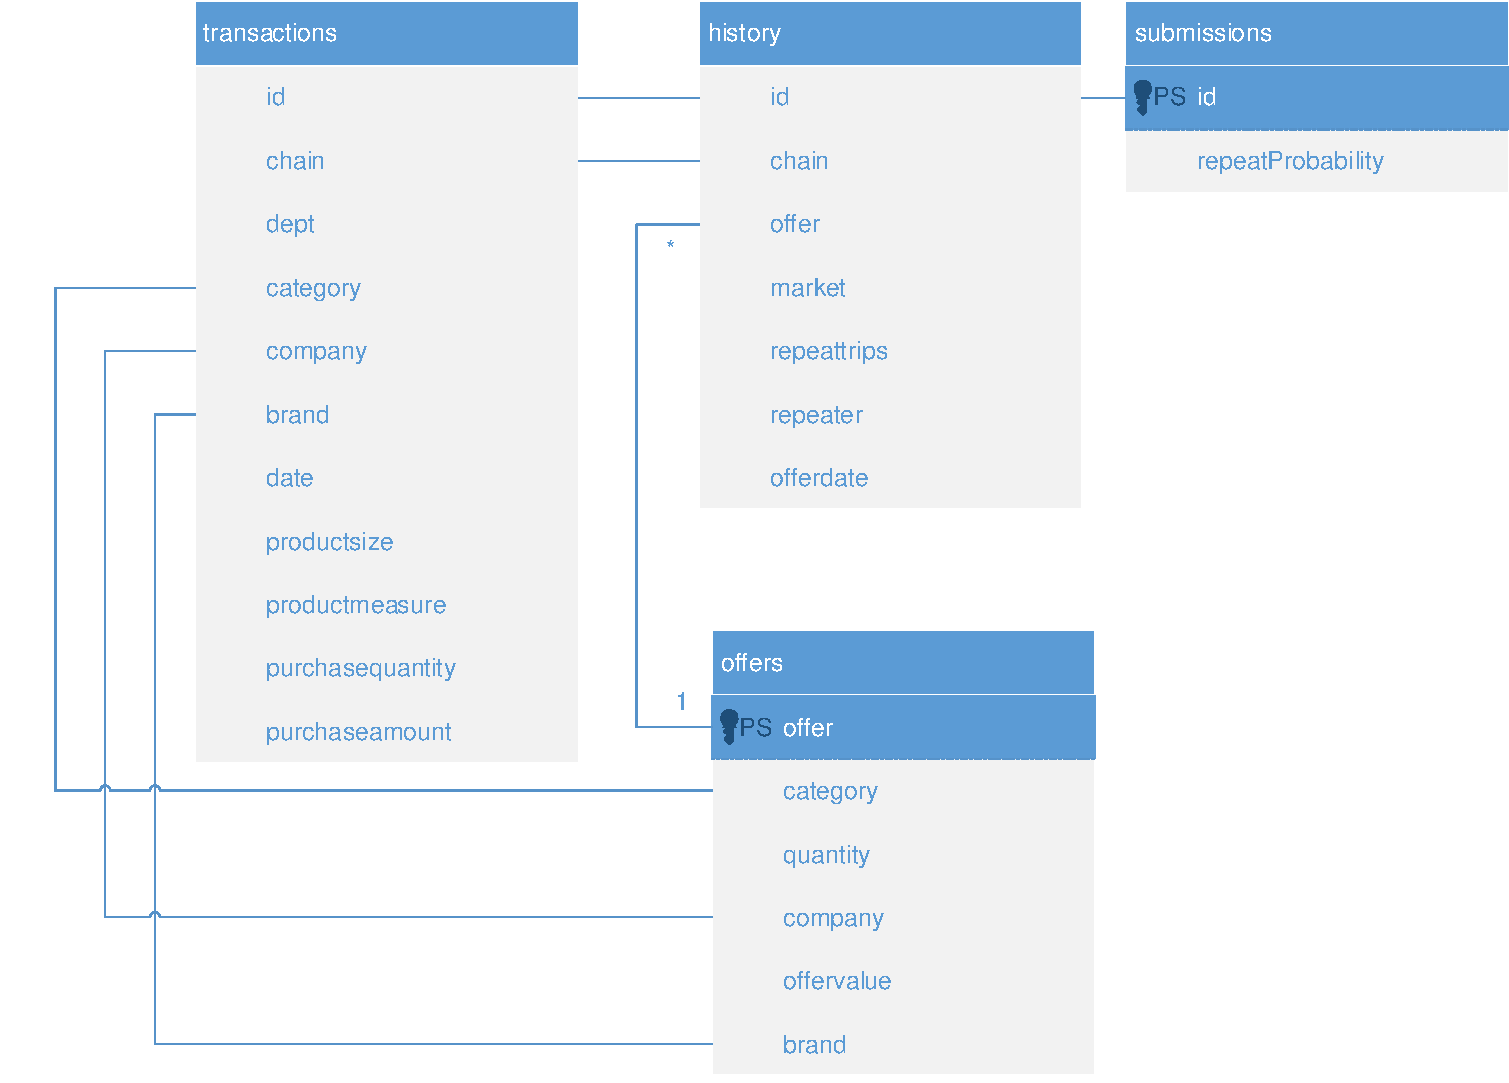
\includegraphics[width=1\linewidth]{Bilder/ShoppersTables}
\caption{Das Datenmodell der Shoppers-Challenge}
\label{fig:ShoppersTables}
\end{figure}

In den "`transactions"' (s. Tabelle \ref{tab:transactions}) stehen die Einkäufe der Kunden.
Die "`offers"' (s. Tabelle \ref{tab:offers}) enthalten Gutscheine, die an den Kunden verteilt wurden.
In der "`train\_history"' (s. Tabelle \ref{tab:trainhistory}) sind Informationen über die angebotenen Coupons enthalten.
Die "`test\_history"' entspricht der "`train\_history"' mit dem Unterschied, dass die beiden Felder "`repeattrips"' und "`repeater"' fehlen. Diese sind absichtlich nicht enthalten, da eine Vorhersage über diese Werte getroffen werden soll.
Die "`submissions"' (s. Tabelle \ref{tab:submissions}) enthalten die Ergebnisse, die wir bei Kaggle einreichen. Dabei wird einem Kunden eine Wiederkaufswahrscheinlichkeit zugeordnet.

Ziel dieses Projekts ist es, die Daten aus den "`transactions"', "`offers"' sowie der beiden Historiendaten zur Generierung von "`submissions"' zu nutzen. Es sollen Vorhersagen für alle Kunden-IDs aus der "`test\_history"' gemacht werden.

\begin{table}[h]
\centering
\begin{tabular}{l|l}
	 \textbf{Feld} & \textbf{Bedeutung}  \\ 
	\hline id & ID des Kunden \\ 
	\hline chain & ID der Marktkette \\ 
	\hline dept  & ID der Produktoberkategorie (z.B. Elektronikgeräte)  \\ 
	\hline category & ID der Produktkategorie (z.B. Smartphones) \\ 
	\hline company & ID der Firma die das Produkt verkauft \\ 
	\hline brand & ID der Marke (z.B. iPhone) \\ 
	\hline date & Kaufdatum \\
	\hline productsize & Menge die gekauft wurde (2L Wasser, 500g Mehl) \\ 	
	\hline productmeasure & Einheit (Liter, Gramm, Stück) \\ 	
	\hline purchasequantity & Stückzahl die gekauft wurde (Drei 2L Flaschen Wasser)
	\vspace{0.3cm} \\ 
\end{tabular}
\caption{transactions}
\label{tab:transactions}
\end{table}

\begin{table}[h]
\centering
\begin{tabular}{l|l}
	\textbf{Feld} & \textbf{Bedeutung}  \\ 
	\hline offer & ID des Coupon \\ 
	\hline category & ID der Produktkategorie \\ 
	\hline quantity & Stückzahl ab der ein Coupon gilt \\ 
	\hline company & ID der Firma die Coupons anbietet \\ 
	\hline offervalue & Preis \\ 
	\hline brand & ID der Marke
	\vspace{0.3cm} \\ 
\end{tabular}
\caption{offers}
\label{tab:offers}
\end{table}

\begin{table}[h]
\centering
\begin{tabular}{l|l}
	\textbf{Feld} & \textbf{Bedeutung}  \\ 
	\hline id & ID des Kunden \\ 
	\hline chain & ID der Marktkette \\ 
	\hline offer  & ID des Coupon  \\ 
	\hline market & ID der Region in der sich der Markt befindet  \\ 
	\hline repeattrips & Anzahl der Wiederholungskäufe (gleiches Produkt)  \\ 
	\hline repeater & Gibt an, ob repeattrips größer 0 ist \\ 
	\hline offerdate & Datum an dem der Kunde den Coupon erhalten hat 
	\vspace{0.3cm} \\ 
\end{tabular} 
\caption{train\_history}
\label{tab:trainhistory}
\end{table}

\begin{table}[h]
	\centering
\begin{tabular}{l|l}
	\textbf{Feld} & \textbf{Bedeutung}  \\ 
	\hline id & ID des Kunden \\ 
	\hline repeatProbability & Wahrscheinlichkeit das der Kunde erneut kauft 
	\vspace{0.3cm} \\
\end{tabular} 
\caption{submissions}
\label{tab:submissions}
\end{table}

\subsection{Technologieentscheidung}
Zu Beginn des Projekts haben wir uns Gedanken über die Auswahl der Technologien gemacht. Zum Zeitpunkt der Einarbeitungsphase haben wir bereits Hive und Pig durch gruppenübergreifende Vorträge kennen gelernt. Darüber hinaus standen uns keine weiteren Optionen zur Verfügung, da alternative Technologien erst zu einem späteren Zeitpunkt vorgestellt worden sind.

Somit beschränkte sich die Technologieentscheidung auf die Wahl zwischen Hive und Pig. Da wir in unserem Projekt ausschließlich Analysen auf strukturierte Daten durchgeführt haben, fiel unsere Entscheidung auf Hive. Der einfache Datenimport in Form von Tabellen und die einfachen Abfragemöglichkeiten in der SQL-ähnlichen Abfragesprache HQL waren die ausschlaggebenden Kriterien.

Die Technologien, die wir neben Hive verwendet haben, werden im weiteren Verlauf der Dokumentation erläutert.


\subsection{Data-Mining-Verfahren}

\section{Realisierung}

Die Implementierung erfolgt iterativ. D.h. wir entwickeln unterschiedliche ggf. aufeinander aufbauende Lösungen
und versuchen uns mit jedem Versuch zu verbessern. Unseren Fortschritt messen wir, indem wir in jeder
Iteration ein einreichbares Ergebnis erzeugen. Die Bewertung erfolgt somit über einen internen Algorithmus
von Kaggle.

Allgemein:
- Erst lokal testen mit kleinen Daten
- Dann auf gesamten Daten in Hive

\subsection{Implementierung}

\subsubsection{Iteration 0}

Als Erstes wollen wir eine Grundlage zur Bewertung folgender Versuche schaffen und das Einreichen einer
Lösung bei Kaggle üben. Dazu erzeugen wir eine Datei, die jedem Kunden die Kaufwahrscheinlichkeit 0\%
zuordnet. Hierzu verwenden wir eine rudimentäre Hive-Abfrage.

\begin{lstlisting}[language=SQL]
SELECT DISTINCT(h.id), 0.0 AS repeatProbability 
FROM test_history h
\end{lstlisting}

Die Bewertung von Kaggle sieht wie folgt aus:

\begin{tabular}{|c|c|}
	\hline \textbf{Platzierung} & \textbf{Bewertung} \\ 
	\hline 932 & 0.50000  \\ 
	\hline 
\end{tabular}

\subsubsection{Iteration 1}

Im nächsten Schritt wollen wir den ersten "`Prior Category Benchmark"' von Kaggle implementieren.
Dieser Benchmark ordnet Kunden, die bereits ein Produkt der Angebotskategorie gekauft haben, die
Wiederkaufwahrscheinlichkeit 1 zu. Allen anderen Kunden wird die Wahrscheinlichkeit 0 zugeordnet.

Wir bestimmen die Kunden mit einer Wahrscheinlichkeit von 1 über folgende Hive-Abfrage:
\begin{lstlisting}[language=SQL]
SELECT DISTINCT h.id, 1.0 AS repeatProbability
FROM test_history h INNER JOIN offers o ON (h.offer = o.offer)
INNER JOIN transactions t ON (t.id = h.id)
WHERE t.category = o.category
\end{lstlisting}

Um das Ergebnis bei Kaggle einzureichen, fehlen noch die Kunden mit einer Wahrscheinlichkeit von 0.
Um diese hinzuzufügen wurde ein Python-Skript entwickelt, dass eine unvollständige Einreichung
um die fehlenden Einträge erweitert. Für diese Kunden wird eine Wahrscheinlichkeit von 0 eingetragen.
Dieses Skript (s. Anhang \ref{code:complete-submission}) kann in weiteren Iterationen verwendet werden,
um sicher zu stellen, dass das Ergebnis vollständig ist und die Überprüfung von Kaggle übersteht. 

Die Bewertung von Kaggle ergibt wie erwartet:

\begin{tabular}{|c|c|}
	\hline \textbf{Platzierung} & \textbf{Bewertung} \\ 
	\hline 747 & 0.52000  \\ 
	\hline 
\end{tabular}

\subsubsection{Iteration 2}

In Iteration 1 haben wir den Benchmark mit der niedrigsten Bewertung implementiert. Jetzt wollen wir 
den besten Benchmark umsetzen. Der "`Prior (Brand \& Company \& Category) Benchmark"' ist sehr ähnlich
zu dem ersten Benchmark. Wir ordnen jedem Kunden, der schon einmal ein Produkt der Angebotsmarke,
des Angebotsunternehmens und der Angebotskategorie gekauft hat, eine 1 zu. Den anderen Kunden wird
eine Wahrscheinlichkeit von 0 zugeordnet.

\begin{lstlisting}[language=SQL]
SELECT DISTINCT h.id, 1.0 AS repeatProbability
FROM test_history h INNER JOIN offers o ON (h.offer = o.offer)
INNER JOIN transactions t ON (t.id = h.id)
WHERE t.category = o.category
  AND t.company = o.company
  AND t.brand = o.brand
\end{lstlisting}

Bevor wir das Ergebnis einreichen, verwenden wir das Skript zum Vervollständigen aus Iteration 1.

\begin{tabular}{|c|c|}
	\hline \textbf{Platzierung} & \textbf{Bewertung} \\ 
	\hline 627 & 0.56425  \\ 
	\hline 
\end{tabular}

\subsubsection{Iteration 3}

Nachdem wir in den vorherigen Iterationen die vorgegeben Benchmarks von Kaggle implementiert haben,
wollen wir jetzt ein richtiges Data-Mining-Verfahren verwenden. Dazu ermitteln wir im ersten Schritt
auf Basis der Transaktionsdaten Features für jeden Kunden. Bei der Wahl der Features orientieren
wir uns an den Ergebnissen von einem Kaggle-Nutzer (\url{http://mlwave.com/predicting-repeat-buyers-vowpal-wabbit/}).

Folgende Merkmale werden jeweils für die Marke (brand), das Unternehmen (company) und die Kategorie (category)
des Angebots (offer) ermittelt:
\begin{itemize}
	\item Für wie viele Produkte mit welchem Preis gilt das Angebot?
	\item Wie oft hat der Kunde in den letzen 30, 60, 90 und 180 Tagen gekauft? (Transaktionszahl)
	\item Wie viel hat der Kunde in den letzen 30, 60, 90 und 180 Tagen gekauft? (Anzahl gekaufter Produkte)
	\item Für wie viel Geld hat der Kunde in den letzen 30, 60, 90 und 180 Tagen gekauft? (Kosten)
\end{itemize}

Die Features werden über eine Reihe von Hive-Abfragen erstellt. Um die Zwischenergebnisse auch für
weitere Iterationen nutzen zu können, legen wir Tabellen mit den Ergebnissen an. Das erlaubt zusätzlich
einen strukturierten Aufbau der Merkmale.

Da die Kunden-Daten verteilt über die \texttt{train\_history} und die \texttt{test\_history} sind, 
bilden wir zuerst die Vereinigung der Kunden-Daten:
\begin{lstlisting}[language=SQL]
CREATE TABLE customers AS 
(
  SELECT te.id, te.offer, te.offerdate
    FROM test_history te
  UNION
  SELECT tr.id, tr.offer, tr.offerdate
    FROM train_history tr 
)
\end{lstlisting}
Danach ermitteln wir die Transaktionsdaten, die sich jeweils auf die Marke, das Unternehmen oder 
die Kategorie des Angebots für den Kunden beziehen. Dabei ermitteln wir zusätzlich, wie viele
Tage vor dem Angebot die Transaktion durchgeführt wurde. Beispielhaft ist hier die Abfrage
für die Marke dargestellt. Die anderen Anfragen werden analog erstellt und sind im Anhang
\ref{sql:filtered_tx} hinterlegt.
\begin{lstlisting}[language=SQL]
CREATE TABLE filtered_tx_brand AS
  SELECT t.id, t.purchasequantity, t.purchaseamount, (c.offerdate - t.date) AS daysbefore 
  FROM transactions t 
  INNER JOIN customers c ON (t.id = c.id)
  INNER JOIN offers o ON (c.offer = o.offer)
  WHERE o.brand = t.brand
\end{lstlisting}

Anschließend werden die gefilterten Transaktionsdaten gruppiert nach
Zeitintervallen ausgewertet. Die vollständigen Abfragen befinden sich
in Anhang \ref{sql:features_bcc}. Hier wird ein Auszug aus der
Abfrage für die Marken-Features dargestellt:
\begin{lstlisting}[language=SQL]
CREATE TABLE category_features AS
SELECT ever.id, ever.tx_count, ever.quantity, ever.cost,
before30.tx_count AS tx_count_30, before30.quantity AS quantity_30, before30.cost AS cost_30,
before60.tx_count AS tx_count_60, before60.quantity AS quantity_60, before60.cost AS cost_60,
before90.tx_count AS tx_count_90, before90.quantity AS quantity_90, before90.cost AS cost_90,
before180.tx_count AS tx_count_180, before180.quantity AS quantity_180, before180.cost AS cost_180
FROM 
(SELECT id, COUNT(*) AS tx_count, SUM(purchasequantity) AS quantity, 
SUM(purchaseamount) AS cost
FROM filtered_tx_category
GROUP BY id
) ever
LEFT JOIN
(SELECT id, COUNT(*) AS tx_count, SUM(purchasequantity) AS quantity, 
SUM(purchaseamount) AS cost
FROM filtered_tx_category
WHERE daysbefore <= 30
GROUP BY id
) before30
ON (ever.id = before30.id)
LEFT JOIN
...
\end{lstlisting}

Jetzt müssen die unterschiedlichen Features nur noch zusammengeführt werden. Dies passiert
in Anhang \ref{sql:features_combined_3} und umfasst einen Join zwischen den
unterschiedlichen Features auf Basis der Kunden-ID.

\begin{tabular}{|c|c|}
	\hline \textbf{Platzierung} & \textbf{Bewertung} \\ 
	\hline 499 & 0.58051  \\ 
	\hline 
\end{tabular}

\subsubsection{Iteration 4}

Feature-Engineerung: Jetzt auch negative Features

Ergänzung zu der Datei, die die Eingabe für Vorpal Wabbit erzeugt:
\begin{lstlisting}[language=Python]
# Negative Features erzeugen, wenn nichts gekauft wurde
if len(row['b_tx_count']) == 0:
	output += ' b_never:1'
if len(row['co_tx_count']) == 0:
	output += ' co_never:1'
if len(row['ca_tx_count']) == 0:
	output += ' ca_never:1'
\end{lstlisting}

\begin{tabular}{|c|c|}
	\hline \textbf{Platzierung} & \textbf{Bewertung} \\ 
	\hline 344 & 0.58786  \\ 
	\hline 
\end{tabular}

Besser als die im letzten Jahr: 452 0.58519

\subsubsection{Iteration 5}

PLatz 240

\subsubsection{Iteration 6}

Mahout


	
\subsection{Amazon Web Services}

\subsubsection{Tabellenanlage}

\subsubsection{Anfragen ausführen}

Anhang mit Skripten


\section{Schlussteil}

\subsection{Ausblick}
Es konnte bereits während des Projektes ein gutes Ergebnis erzielt
werden. Dennoch wurden aufgrund der knappen Zeit nicht alle Ideen
umgesetzt. Weitere Möglichkeiten sehen wir im Bereich der nicht
verwendeten Daten und der Nutzung eines Offline-Learning-Verfahrens.
Des Weiteren besteht die Möglichkeit, die verwendeten Features auf ihre
Aussagekraft beziehungsweise Qualität zu untersuchen.

\subsubsection{Verwendung aller Daten}
Es werden bisher hauptsächlich Transaktionen berücksichtigt, die in Beziehung zu Gutscheinen stehen.
Bei diesen Transaktionen muss die Marke, die Kategorie oder das Unternehmen mit dem entsprechenden Gutschein übereinstimmen.
Diese Daten könnten in einem nächsten Iterationsschritt ebenfalls verwertet werden, wozu zunächst die folgenden Ansätze zusammengetragen wurden:
	
\begin{itemize}
\item Für jeden Kunden soll der komplette Umsatz pro Quartal bzw. pro Jahr ermittelt werden. Die Idee ist, dass Kunden, die viel Geld umsetzen, weniger gut durch Gutscheine ansprechbar sind, als die Kunden, die wenig zum Umsatz beitragen. 
 
\item Kunden, die in regelmäßigen Abständen einkaufen, kommen sehr wahrscheinlich wieder.
Beispielsweise werden wöchentlich die Nahrungsvorräte auf dem Heimweg von der Arbeit aufgefüllt.
Die Frequenz des Einkaufens kann über die Auswertung der Zeitangaben der Transaktionen ermittelt werden.

\item Clustering von oft zusammen gekauften Marken, Kategorien und Unternehmen. Auf dieser Basis können Features für die Kunden definiert werden.
	
\item Kunden, die große Mengen gekauft haben, kommen wahrscheinlich wieder. Sie benötigen allerdings keine Gutscheine, da der Preis für sie bereits in Ordnung ist oder der Markt beispielsweise zum Einkauf gut gelegen ist. Für eine Umsetzung gilt es eine Definition für "große Menge" zu finden.  Denkbar wäre große Menge als überdurchschnittlich zu definieren, was sich einfach implementieren ließe.
\end{itemize}

\subsubsection{Bewertung von Features}	
Sowohl bei den verwendeten Features als auch bei den oben vorgestellten Ideen ist bisher unklar, inwiefern diese Features das Kaufverhalten positiv, negativ oder überhaupt beeinflussen.
In unseren Vorträge zur Veranstaltung ist zur Sprache gekommen, dass statistische Auswertungsverfahren zur Verfügung stehen, welche Aufschluss über die Qualität der Features treffen können. Da schlechte Features das Ergebnis negativ verfälschen können, ist dieser Ansatz besonders interessant.
Zur Umsetzung müsste die Korrelation zwischen den einzelnen Features und dem Wiederkaufverhalten gemessen werden. Auf dieser Basis kann ein Grenzwert festgelegt werden, ab dem ein Feature
zur Voraussage genutzt wird.

\subsubsection{Offline-Learning-Verfahren}	
Die Trainingsdaten, die von Kaggle für die Aufgabenstellung bereitgestellt werden, sind konstant und werden 
nicht um neue Trainingsdaten erweitert. Daher ist es nicht zwingend notwendig, dass diese inkrementell gelernt
werden. Zurzeit nutzen wir allerdings ein Online-Learning-Verfahren zur Erstellung des Modells. Wie im Kapitel
\nameref{subsubSec:MachineLearning} beschrieben, hat dies zum Nachteil, dass die Reihenfolge, in der die Trainingsdaten
eingelesen werden, Einfluss auf die Generierung des Modells haben. Daher wäre es wünschenswert ein Offline-Learning-Verfahren
anstelle des von uns benutzten Online-Learning-Verfahrens zu nutzen. Aufgrund der begrenzten Zeit, die uns zur 
Lösung des Problems zur Verfügung stand, haben wir keine Implementierung eines Offline-Learning-Verfahrens vollständig 
ausprobieren können. Dies wäre somit ein Punkt bei dem wir uns noch Verbesserungspotenzial erhoffen.

\subsection{Fazit}


\appendix
\section{Hive-Abfragen}

\subsection{Kunden-Daten}
\begin{lstlisting}[language=SQL]
CREATE TABLE customers AS 
(
  SELECT te.id, te.offer, te.offerdate
    FROM test_history te
  UNION
  SELECT tr.id, tr.offer, tr.offerdate
    FROM train_history tr 
)
\end{lstlisting}

\subsection{Transaktionen gefiltert nach Marke, Unternehmen oder Kategorie}
\label{sql:filtered_tx}
\begin{lstlisting}[language=SQL]
-- Gefiltert nach Marke (brand)
CREATE TABLE filtered_tx_brand AS
  SELECT t.id, t.purchasequantity, t.purchaseamount, 
         (c.offerdate - t.date) AS daysbefore 
  FROM filtered_transactions t 
  INNER JOIN customers c ON (t.id = c.id)
  INNER JOIN offers o ON (c.offer = o.offer)
  WHERE o.brand = t.brand
  
-- Gefiltert nach Unternehmen (company)
CREATE TABLE filtered_tx_company AS
  SELECT t.id, t.purchasequantity, t.purchaseamount, 
         (h.offerdate - t.date) AS daysbefore 
  FROM transactions t 
  INNER JOIN test_history h ON (t.id = h.id)
  INNER JOIN offers o ON (h.offer = o.offer)
  WHERE o.company = t.company
  
-- Gefiltert nach Kategorie (category)
CREATE TABLE filtered_tx_category AS
  SELECT t.id, t.purchasequantity, t.purchaseamount, 
         (c.offerdate - t.date) AS daysbefore 
  FROM transactions t 
  INNER JOIN customers c ON (t.id = c.id)
  INNER JOIN offers o ON (c.offer = o.offer)
  WHERE o.category = t.category
\end{lstlisting}

\subsection{Features bezogen auf Marke, Unternehmen oder Kategorie}
\label{sql:features_bcc}
\begin{lstlisting}[language=SQL]
CREATE TABLE category_features AS
SELECT ever.id, ever.tx_count, ever.quantity, ever.cost,
before30.tx_count AS tx_count_30, before30.quantity AS quantity_30, before30.cost AS cost_30,
before60.tx_count AS tx_count_60, before60.quantity AS quantity_60, before60.cost AS cost_60,
before90.tx_count AS tx_count_90, before90.quantity AS quantity_90, before90.cost AS cost_90,
before180.tx_count AS tx_count_180, before180.quantity AS quantity_180, before180.cost AS cost_180
FROM 
(SELECT id, COUNT(*) AS tx_count, SUM(purchasequantity) AS quantity, 
 SUM(purchaseamount) AS cost
 FROM filtered_tx_category
 GROUP BY id
) ever
LEFT JOIN
(SELECT id, COUNT(*) AS tx_count, SUM(purchasequantity) AS quantity, 
 SUM(purchaseamount) AS cost
 FROM filtered_tx_category
 WHERE daysbefore <= 30
 GROUP BY id
) before30
ON (ever.id = before30.id)
LEFT JOIN
(SELECT id, COUNT(*) AS tx_count, SUM(purchasequantity) AS quantity, 
 SUM(purchaseamount) AS cost
 FROM filtered_tx_category
 WHERE daysbefore <= 60
 GROUP BY id
) before60
ON (ever.id = before60.id)
LEFT JOIN
(SELECT id, COUNT(*) AS tx_count, SUM(purchasequantity) AS quantity, 
 SUM(purchaseamount) AS cost
 FROM filtered_tx_category
 WHERE daysbefore <= 90
 GROUP BY id
) before90
ON (ever.id = before90.id)
LEFT JOIN 
(SELECT id, COUNT(*) AS tx_count, SUM(purchasequantity) AS quantity, 
 SUM(purchaseamount) AS cost
 FROM filtered_tx_category
 WHERE daysbefore <= 180
 GROUP BY id
) before180
ON (ever.id = before180.id)
\end{lstlisting}

\subsection{Features kombinieren (Iteration 3)}
\label{sql:features_combined_3}
\begin{lstlisting}[language=SQL]
-- Features der Kunden, für die Vorhersagen gemacht werden sollen
CREATE TABLE test_features AS
  SELECT 
    h.id, 'u' AS repeater,
    o.quantity AS o_quantity, o.offervalue,

    b.tx_count AS b_tx_count, b.quantity AS b_quantity, b.cost AS b_cost,
    b.tx_count_30 AS b_tx_count_30, b.quantity_30 AS b_quantity_30, b.cost_30 AS b_cost_30,
    b.tx_count_60 AS b_tx_count_60, b.quantity_60 AS b_quantity_60, b.cost_60 AS b_cost_60,
    b.tx_count_90 AS b_tx_count_90, b.quantity_90 AS b_quantity_90, b.cost_90 AS b_cost_90,
    b.tx_count_180 AS b_tx_count_180, b.quantity_180 AS b_quantity_180, b.cost_180 AS b_cost_180,

    co.tx_count AS co_tx_count, co.quantity AS co_quantity, co.cost AS co_cost,
    co.tx_count_30 AS co_tx_count_30, co.quantity_30 AS co_quantity_30, co.cost_30 AS co_cost_30,
    co.tx_count_60 AS co_tx_count_60, co.quantity_60 AS co_quantity_60, co.cost_60 AS co_cost_60,
    co.tx_count_90 AS co_tx_count_90, co.quantity_90 AS co_quantity_90, co.cost_90 AS co_cost_90,
    co.tx_count_180 AS co_tx_count_180, co.quantity_180 AS co_quantity_180, co.cost_180 AS co_cost_180,

    ca.tx_count AS ca_tx_count, ca.quantity AS ca_quantity, ca.cost AS ca_cost,
    ca.tx_count_30 AS ca_tx_count_30, ca.quantity_30 AS ca_quantity_30, ca.cost_30 AS ca_cost_30,
    ca.tx_count_60 AS ca_tx_count_60, ca.quantity_60 AS ca_quantity_60, ca.cost_60 AS ca_cost_60,
    ca.tx_count_90 AS ca_tx_count_90, ca.quantity_90 AS ca_quantity_90, ca.cost_90 AS ca_cost_90,
    ca.tx_count_180 AS ca_tx_count_180, ca.quantity_180 AS ca_quantity_180, ca.cost_180 AS ca_cost_180

  FROM test_history h
  INNER JOIN offers o ON (h.offer = o.offer)
  LEFT JOIN brand_features b ON (h.id = b.id)
  LEFT JOIN company_features co ON (h.id = co.id)
  LEFT JOIN category_features ca ON (h.id = ca.id)

-- Features der Kunden, für die Wiederkaufsdaten bekannt sind
CREATE TABLE train_features AS
  SELECT 
    h.id, h.repeater,
    o.quantity AS o_quantity, o.offervalue,

    b.tx_count AS b_tx_count, b.quantity AS b_quantity, b.cost AS b_cost,
    b.tx_count_30 AS b_tx_count_30, b.quantity_30 AS b_quantity_30, b.cost_30 AS b_cost_30,
    b.tx_count_60 AS b_tx_count_60, b.quantity_60 AS b_quantity_60, b.cost_60 AS b_cost_60,
    b.tx_count_90 AS b_tx_count_90, b.quantity_90 AS b_quantity_90, b.cost_90 AS b_cost_90,
    b.tx_count_180 AS b_tx_count_180, b.quantity_180 AS b_quantity_180, b.cost_180 AS b_cost_180,

    co.tx_count AS co_tx_count, co.quantity AS co_quantity, co.cost AS co_cost,
    co.tx_count_30 AS co_tx_count_30, co.quantity_30 AS co_quantity_30, co.cost_30 AS co_cost_30,
    co.tx_count_60 AS co_tx_count_60, co.quantity_60 AS co_quantity_60, co.cost_60 AS co_cost_60,
    co.tx_count_90 AS co_tx_count_90, co.quantity_90 AS co_quantity_90, co.cost_90 AS co_cost_90,
    co.tx_count_180 AS co_tx_count_180, co.quantity_180 AS co_quantity_180, co.cost_180 AS co_cost_180,

    ca.tx_count AS ca_tx_count, ca.quantity AS ca_quantity, ca.cost AS ca_cost,
    ca.tx_count_30 AS ca_tx_count_30, ca.quantity_30 AS ca_quantity_30, ca.cost_30 AS ca_cost_30,
    ca.tx_count_60 AS ca_tx_count_60, ca.quantity_60 AS ca_quantity_60, ca.cost_60 AS ca_cost_60,
    ca.tx_count_90 AS ca_tx_count_90, ca.quantity_90 AS ca_quantity_90, ca.cost_90 AS ca_cost_90,
    ca.tx_count_180 AS ca_tx_count_180, ca.quantity_180 AS ca_quantity_180, ca.cost_180 AS ca_cost_180

  FROM train_history h
  INNER JOIN offers o ON (h.offer = o.offer)
  LEFT JOIN brand_features b ON (h.id = b.id)
  LEFT JOIN company_features co ON (h.id = co.id)
  LEFT JOIN category_features ca ON (h.id = ca.id)
\end{lstlisting}

\section{complete-submission.py}
\label{code:complete-submission}
\begin{lstlisting}[language=Python]
#!/usr/bin/env python

# Diese Skript vervollständigt eine Kaggle-Einreichung.
# Fehlenden Kunden wird eine Wahrscheinlichkeit von 0 
# zugeordnet.
# Die Datei sampleSubmissions.csv muss sich im aktuellen 
# Verzeichnis befinden

import sys

samplesFile = open('sampleSubmission.csv', 'r')
samplesFile.readline()
samples = { }
for line in samplesFile:
	id, prob = line.split(',', 1)
	samples[id] = prob

# Erste Zeile ignorieren
sys.stdin.readline()
# Und die geforderte Kopfzeile ausgeben
sys.stdout.write("id,repeatProbability\n")

for line in sys.stdin:
	id, prob = line.split(',', 1)
	if (id in samples):
		del samples[id]
	sys.stdout.write(id + ',' + prob)

	for id in samples:
		sys.stdout.write(id + ',' + samples[id])
\end{lstlisting}

\section{features-to-vw.py}
\label{code:features-to-vw}
\begin{lstlisting}[language=Python]
#!/usr/bin/env python

import sys
import csv

input = csv.DictReader(sys.stdin, delimiter=',')
for row in input:
	# Ausgabe beginnt mit der Klassifizierung:
	# hat gekauft (1), hat nicht gekauft (0) oder unbekannt (0.5)
	output = '0.5'
	if row['repeater'] == 't':
		output = '1'
	elif row['repeater'] == 'f':
		output = '0'

	# Customer ID eintragen und Feature-Liste beginnen
	output += ' \'' + row['id'] + ' |f'

	# Spalten in Features übersetzen
	for key in row:
		if key != 'id' and  key != 'repeater' and len(row[key]) > 0:
			output += ' ' + key + ':' + row[key]

	print(output)
\end{lstlisting}

\section{vw-preds-to-csv.py}
\label{code:vw-preds-to-csv}
\begin{lstlisting}[language=Python]
#!/usr/bin/env python

import sys

# Das Ergebnis von Vorpal Wabbit gibt ein Paar aus 
# Wahrscheinlichkeit und Kunden-ID pro Zeile und durch ein
# Leerzeichen getrennt aus.
# Dieses Programm konviertiert diese Format in da von Kaggle
# geforderte CSV-Format.

print('id,repeatProbability')

for line in sys.stdin:
	prob, id = line.split(' ', 1)
	print(id[:-1] + ',' + prob)
\end{lstlisting}
	
	

\newpage
%\printbibliography

\end{document}